\documentclass[paper=a4, fontsize=11pt, ngerman, abstract=on]{scrartcl}

\usepackage{tocloft}
\usepackage{titling}
\usepackage{blindtext}
\usepackage{subcaption}
\usepackage[utf8]{inputenc}
\usepackage[T1]{fontenc}
\usepackage[ngerman]{babel}
\usepackage{amsmath,amsfonts,amsthm}
\usepackage{siunitx}
\sisetup{output-decimal-marker = {,}}
\usepackage{graphicx}

\usepackage{sectsty}
\allsectionsfont{\raggedright \normalfont\scshape}

\usepackage{fancyhdr}
\pagestyle{fancyplain}

\fancyhead{} % Head Footer
\fancyfoot[L]{} % Left Footer
\fancyfoot[C]{} % Center Footer
\fancyfoot[R]{\thepage} % Right Footer - Page numbering
\renewcommand{\headrulewidth}{0pt} % Remove header underlines
\renewcommand{\footrulewidth}{0pt} % Remove footer underlines
\setlength{\headheight}{13.6pt} % Customize the height of the header

\numberwithin{equation}{section} % Number equations within sections (i.e. 1.1, 1.2, 2.1, 2.2 instead of 1, 2, 3, 4)
\numberwithin{figure}{section} % Number figures within sections (i.e. 1.1, 1.2, 2.1, 2.2 instead of 1, 2, 3, 4)
\numberwithin{table}{section} % Number tables within sections (i.e. 1.1, 1.2, 2.1, 2.2 instead of 1, 2, 3, 4)

\setlength\parindent{0pt} % Removes all indentation from paragraphs - comment this line for an assignment with lots of text

\newcommand {\horrule}[1]{\rule{\linewidth}{#1}} % Create horizontal rule command with 1 argument of height

\usepackage{listings}
\usepackage{color}

\definecolor{mygreen}{RGB}{28,172,0}
\definecolor{mylilas}{RGB}{170,55,241}
\lstdefinestyle{matlab}{language=Matlab,%
  breaklines=true,%
  morekeywords={matlab2tikz},
  keywordstyle=\color{blue},%
  morekeywords=[2]{1}, keywordstyle=[2]{\color{black}},
  identifierstyle=\color{black},%
  stringstyle=\color{mylilas},
  commentstyle=\color{mygreen},%
  showstringspaces=false,%without this there will be a symbol in the places where there is a space
  basicstyle=\footnotesize,
  stepnumber=1,
  emph=[1]{for,end,break},emphstyle=[1]\color{blue},
  % frame=tb,
  rulesepcolor=\color{black},
  rulecolor=\color{black},
  framesep=3pt,
  xleftmargin=3pt,
  xrightmargin=8pt,
  tabsize=2
}

\definecolor{deepblue}{rgb}{0,0,0.5}
\definecolor{deepred}{rgb}{0.6,0,0}
\definecolor{deepgreen}{rgb}{0,0.5,0}
\lstdefinestyle{python}{language=Python,%
  breaklines=true,%
  otherkeywords={self},
  morekeywords={},
  keywordstyle=\color{deepblue},%
  morekeywords=[2]{1}, keywordstyle=[2]{\color{black}},
  identifierstyle=\color{black},%
  stringstyle=\color{deepgreen},
  commentstyle=\color{black},%
  showstringspaces=false,%without this there will be a symbol in the places where there is a space
  basicstyle=\footnotesize,
  stepnumber=1,
  emph={MyClass,__init__,for,in,break,continue,try,except},
  emphstyle=\color{deepred},
  frame=tb,
  rulesepcolor=\color{black},
  rulecolor=\color{black},
  framesep=3pt,
  xleftmargin=3pt,
  xrightmargin=8pt,
  tabsize=2
}

\title {
  \normalfont \normalsize
  \textsc{HAW Hamburg} \\ [25pt]
  \textsc{Modellierung Dynamischer Systeme} \\ [15pt]
  \horrule{0.5pt} \\[0.4cm] % Thin top horizontal rule
  \huge Ausbreitung von Tuberkulose \\ [15pt] % The assignment title
  \small Ein Populationsmodell \\ [15pt]
  \small Prof. Dr. Fohl \\
  \horrule{1pt} \\[0.5cm] % Thick bottom horizontal rule
}

\author{
  Matthias Nitsche \\
  \texttt{matthias.nitsche@haw-hamburg.de} \\
  \small{Hamburg University of Applied Sciences, Department of Computer Science} \\
  \small{Berliner Tor 7} \\
  \small{20099 Hamburg, Germany} \\
}

\begin{document}

\maketitle

\renewcaptionname{ngerman}{\abstractname}{Kurzfassung}
\begin{abstract}
In dieser Arbeit wird eine Übersicht von mathematischen Analyseverfahren zur Übertragung von Tuberkulose präsentiert. Hierzu zählen die Compartment Modelle wie SEIR und agentenbasierte Modelle (ABM). Tuberkulose ist eine komplexe Erkrankung mit unterschiedlichen Krankheitsstadien. Das Ziel von derartigen Modellierungen ist das Identifizieren von optimalen Parametern, sodass ein teil der Realität dargestellt werden kann. Dies führt idealerweise zu neuen Erkenntnissen wie z. B. durch Impfung, Tuberkulose langfristig verhindert werden kann. Auf dem Weg wird der Einfluss von Impfung, Immunerkrankungen, Alter und Lokalität untersucht. Modelle dieser Arbeit wurden mithilfe von Matlab und Python Mesa realisiert.
\end{abstract}

\newpage

\renewcommand{\cftsecleader}{\cftdotfill{\cftdotsep}}
\tableofcontents

\newpage

\section{Domäne - Tuberkulose}

Tuberkulose ist eine bakterielle Infektionserkrankung, die besonders häufig die Lunge befällt. Die WHO gibt Tuberkulose als eine der top 10 Todesursachen der Welt an, mit einer Sterberate von 1.8 Millionen Menschen und 10.4 Millionen Neuinfektionen in 2015. Es ist ein aktives Sustainable Development Goal (SDG) das bis 2030 eingedämpft werden soll. Tuberkulose ist eine Krankheit die in Ländern mit schlechter medizinischer Versorgung und tropischem Klima (Sonne und starker Regen) gesondert auftritt. \cite{WHOTB2016}

\subsection{Krankheitsbild}

Tuberkulose (TB) wird vor allem über die Luft übertragen. Das Befallen der Lungen resultiert nicht zwangsweise in einer aktiven Infektion der Krankheit. In Abbildung \ref{fig:tuberculosis-cycle} ist der Kreislauf der Tuberkulose Übertragung.

\begin{figure}[ht]
\centering
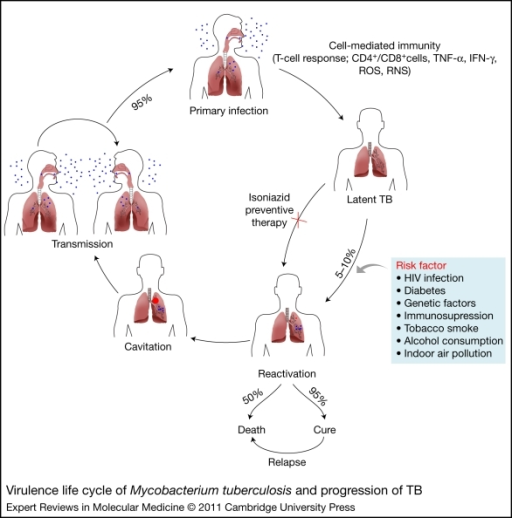
\includegraphics[width=0.5\textwidth,keepaspectratio]{images/tuberculosis-cycle}
\caption{Tuberkulose Kreislauf in \cite{Kumar2011}}
\label{fig:tuberculosis-cycle}
\end{figure}

In kurz, ein Mensch wird über direkten Kontakt von einem anderen über die Luft mit Tuberkulose latent infiziert, hat wesentlich geringere Wahrscheinlichkeit infiziert zu werden und eine hohe Wahrscheinlichkeit bei nicht Medikation zu sterben.

\begin{enumerate}
\item{Die \textbf{Übertragung} findet über die Luft zwischen zwei Menschen statt. Häufig ist deshalb der Ort der Übertragung in Lebensgemeinschaften auf engem Raum, öffentlichen Verkehrsmitteln oder Arbeitsplätzen. Klimaanlagen beschleunigen die Verbreitung von Bakterien in der Luft. Bei direktem Kontakt ist die Wahrscheinlichkeit auf Ansteckung bei 95\% und es wird eine Hauptinfektion ausgelöst.}
\item{Die \textbf{Hauptinfektion} ist meist ein befallen der Lunge. Verschiedene Immunfaktoren beeinflussen die Geschwindigkeit des Fortschreitens.}
\item{Betroffene sind ab diesem Schritt \textbf{latent infiziert}. Während das Subjekt in der latenten TB Phase ist, tauchen nicht zwangsweise Symptome auf. Die meisten latent infizierten Träger von TB haben in ihrem ganzen Leben keinerlei Auswirkungen der Krankheit. In dem latenten Stadium können Subjekte niemanden anstecken. Einige Faktoren beeinflussen jedoch die Wahrscheinlichkeit auf eine aktive Infektion, sogenannte Risikofaktoren. Diese sind vor allem Immunbedingt wie z. B. HIV, Diabetes, genetische Faktoren, Immunsupressiver und viele mehr. Subjekte mit derartigen Ausprägungen haben eine Wahrscheinlichkeit von 5 bis 10\% die Krankheit als aktive Infektion zu entwickeln. In den Fällen wo eine Präventivtherapie nicht hilft erfolgt meist eine aktive Krankheitsentwicklung.}
\item{Die \textbf{aktive Infektion/Reaktivierung} erfolgt irgendwann, nachdem ein Subjekt latent infiziert wurde. Ab diesem Punkt gibt es nur zwei Möglichkeiten, Menschen die eine Heilung bekommen werden zu 95\% wieder gesund. 50\% die keine Heilung bekommen sterben und 50\% bessern sich von selbst. Ein Rückfall führt meistens zum Tode. Infizierte sind ab jetzt Überträger der Krankheit. Menschen die von TB geheilt werden gehen zurück ins latente Stadium. Eine vollständige Heilung ist nicht mehr möglich.}
\end{enumerate}

An diesem Model wird relativ schnell klar, warum TB so gefährlich ist. Betroffene können nie wieder von der Krankheit regenerieren und Immunfaktoren, die besonders im Alter schlechter werden, begünstigen den Ausbruch der Krankheit. Zudem kommt das TB in zwei Formen auftritt. TB als herkömliche, behandelbare Erkrankung und Multi-Drug-Resistant TB (MDR-TB), bei der TB ressistent gegenüber den derzeitig stärksten Medikationen ist. Tatsächlich ist nach der WHO die MDR-TB Erkrankungen am Steigen.

\subsection{Behandlung}

Die Behandlung von TB kann vielschichtig erfolgen. Häufig eignet sich eine Impfung direkt bei der Geburt, aber auch später bei bisheriger nicht Erkrankung. Besondere Maßnahmen müssen bei TB und HIV berücksichtigt werden. Die Inzidenzrate von TB ist fast endemisch bei Trägern von HIV. Da HIV über Blut oder Körpersekrete weitergegeben wird, sind vor allem Länder betroffen, wo es einen hohen Teil an HIV infizierten gibt, schlechte Aufklärung und Mittel zur Verhütung. In Regionen wo TB bereits als Epidemie ausgebrochen ist, muss die Bevölkerung aufgeklärt werden, sodass gegenschritte eingeleitet werden können. Zentren für Medikation, Behandlungen von Erkrankten und Isolation von der gesunden Bevölkerung. Isolation ist hier besonders wichtig, sowohl für nicht erkrankte als auch erkrankte. Betroffene Regionen müssen gewarnt werden, sodass erkrankte selbstständig Hilfe suchen und nicht Betroffene nur für die wichtigsten Fälle in die Öffentlichkeit gehen. Individuen können außerdem durch Gesundheitsfaktoren wie Nahrung und geringen Konsum von Zigaretten oder Alkohol höhere Wahrscheinlichkeiten auf nicht Infektion haben. \cite{WHOTBGuidelines2017}

\subsection{Faktoren}

Es gibt einige Faktoren, die besonders gut die Ausbreitung von Tuberkulose beschreiben können. Dazu gehören

\begin{itemize}
\item Die Abdenkung von Impfung in der Bevölkerung
\item Immunerkrankungen wie HIV oder Diabetes
\item Alter
\item Alkohol und Zigarettenkonsum
\item Lebensraum in quadratmeter pro Individuum
\item Transport (Flugzeug oder Schiff) und öffentliche Verkehrsmittel (Bus oer Bahn)
\item Regen und Hitze (tropisches Klima)
\item Gruppierungen von Menschen (z. B. durchschnittliche Größe und Menge an Unternehmen, durchschnittlie Familiengröße, öffentliche Plätze)
\item TB resistent gegen Medikation (MDR-TB)
\end{itemize}

Häufig lassen sich diese Faktoren aus Berichten der WHO und weiteren extrahieren. So ist es möglich eine Bevökerung anhand dieser Faktoren als Durchschnitt der Bevölkerung zu modellieren. Das Erkennen und aufdecken dieser Variablen ist enorm wichtig. Die aufgelisteten Faktoren sind die wichtigsten und offensichtlichsten Faktoren. Es gibt dutzende weitere die auf den ersten Blick nicht erkenntlich sind und eventuell hervorragende Prädiktoren für TB sind. \cite{WHOTB2016}

\subsection{Ausbreitung von Infektionskrankheiten}

Die Modellierung der Ausbreitung von Tuberkulose gehört zu einer höheren Kategorie von Modellen der Ausbreitung von Infektionskrankheiten. Infektionskrankheiten sind nach der Epidemiologie, Erkankungen die durch einen Erreger hervorgerufen werden, die meist parasitär in einem Wirt Leben und transient (kurze Dauer, hohe Infektion) oder persistent (lange Dauer, niedrige Infektion) auftreten. Sie gehen in der Regel mit starken septischen Symptonem einher, wenn eine aktive Phase eintritt. \\

Bei der Modellierung der Ausbreitung von Infektionskrankheiten wird in drei Modellen unterschieden. Diese Modelle sind nicht zwingend diskret, da es viele Überlappungen geben kann.

\begin{enumerate}
\item{\textbf{Compartment Modelle} sind solche in denen Individuen einer Bevölkerung in Klassen eingeordnet werden. Die Standardklassen beinhalten Subsceptibles (Empfänger), Exposed (latent infizierte), Infected (Infizifert) und Recovered (Erholte).}
\item{\textbf{Statistische Modelle} schauen sich historische Daten von Bevölkerungen an wo TB aufgetreten ist. Mithilfe dieser Daten können z.B. Prädiktionsmodelle entwickelt werden, um vorhersagen, wo die nächste TB Epidemie ausbricht.}
\item{\textbf{Agentenbasierte Modellierung} modelliert jedes einzelne Individuum aufgrund von Bevölkerungsparametern und lässt diese auf Grids miteinander interagieren. Der Vorteil zu reinen Compartment Modellen ist das die Lokalität der einzelnen Agenten eine Rolle spielt. Der Nachteil, dass große Simulation enorme Rechenleistung erfordern.}
\end{enumerate}

Im Folgenden werden die Compartment Modelle und die agentenbasierte Modellierung am Beispiel von Tuberkulose beschrieben und erläutert.

\section{Compartment Modelle zur Ausbreitung von Tuberkulose}

Compartment Modelle werden über Differentialgleichungssysteme beschrieben. Das einfachste dieser Modelle ist das Susceptible-Infected-Recovered (SIR) Modell. Die Bevölkerungspopulation wird durch $N = S + I + R$ zu einem Zeitpunkt $t$ evaluiert. Diese Werte werden durch das Differentialgleichungssystem \ref{eq:dgls-sir} zu einem Zeitpunkt $t$, über ein Zeitintervall mit einer fixen Schrittweite approximiert. \cite{MathOfInfectiousDiseases2000}

\begin{equation}
\begin{split}
\frac{dS}{dt} &= \mu N - \mu S - \beta \frac{I}{N}S \\
\frac{dI}{dt} &= \beta \frac{I}{N}S - (\gamma + \mu)I \\
\frac{dR}{dt} &= \gamma I - \mu R
\end{split}
\label{eq:dgls-sir}
\end{equation}

Die Parameter des SIR Modells sind $\mu$ die Sterberate, $\beta$ die Infektionsrate und $\gamma$ die Erholungsrate. Die Sterberate ist die generelle Sterberate in der Bevölkerung. Für ein realeres, kontinuierliches Modell mit Zyklen, bräuchte dieses Modell auch einen entsprechenden Geburtenratenparameter. Das vorliegende einfache $SIR$ Modell ist ein

\begin{itemize}
\item{gewönhliches Differentialgleichungssystem}
\item{erster Ordnung}
\item{welches nicht-linear ist, durch $\frac{I}{N}S$, da $S$ nicht mit einer Konstanten multipliziert wird. Dadurch sind keine einfachen analytischen Lösungen möglich. Allerdings konnte \cite{Harko2014} eine exakte Lösung für das $SIR$ Modell präsentieren.}
\end{itemize}

Das SIR Modell kann leicht durch latent infizierte (Exposed) zum SEIR Modell erweitert werden. Das Differentialgleichungssystem \ref{eq:dgls-seir} bekommt eine zusätzliche Klasse $E$ mit dem korrespondierenden Zunahmeparameter $\alpha$, wobei $N = S + E + I + R$ gilt. Auch hier nimmt $E$ um $(\alpha + \mu)$ in $I$ ab und steigt um $\gamma I$, die Abnahme der infizierten, an. \cite{MathOfInfectiousDiseases2000}

\begin{equation}
\begin{split}
\frac{dS}{dt} &= \mu N - \mu S - \beta \frac{I}{N}S \\
\frac{dE}{dt} &= \beta \frac{I}{N}S - (\alpha + \mu)E \\
\frac{dI}{dt} &= \alpha E - (\gamma + \mu)I \\
\frac{dR}{dt} &= \gamma I - \mu R
\end{split}
\label{eq:dgls-seir}
\end{equation}

Die Übergangsparameter mit den zugehörigen Compartments stellen Übergangswahrscheinlichkeiten zwischen den Compartments dar. Sollte es z.B. möglich sein direkt von $S$ zu $I$ zu laufen, kann ein entsprechender Zunahmeparameter einfügt werden. Das letzte und vollständigste Differentialgleichungssystem MSEIRS in \ref{eq:dgls-mseirs} stellt eine relativ nahe Modellierung von Tuberkulose dar.

\begin{equation}
\begin{split}
\frac{dM}{dt} &= N - \sigma M - \mu M \\
\frac{dS}{dt} &= \sigma M - \mu S - \rho(t)\beta \frac{I}{N}S \\
\frac{dE}{dt} &= \beta \frac{I}{N}S - \rho(t)(\alpha + \mu)E + \lambda R \\
\frac{dI}{dt} &= \rho(t)\alpha E - (\gamma + \mu)I \\
\frac{dR}{dt} &= \gamma I - (\mu + \lambda) R
\end{split}
\label{eq:dgls-mseirs}
\end{equation}

In diesem Differentialgleichungssystem wurden drei zusätzliche Modifikationen unternommen.

\begin{enumerate}
\item{Es wurde eine Klasse von geimpften $M$ bei der Geburt eingefügt die mit einer Wahrscheinlichkeit von $\sigma$ nach $S$ gehen können.}
\item{Es gibt einen direkten Weg von $R$ zu $E$ mit einer Wahrscheinlichkeit $\lambda$.}
\item{Es wurde ein variierender Zeitparameter $\rho (t)$ eingefügt, um saisonale Schwankungen zu berücksichtigen. Dieser könnte z. B. $1/365$ für 1 Tag pro Berechnung darstellen. Dies müsste im Fall der Tuberkulose, deutlich genauer modelliert werden, da diese vor allem in heißen regnerischen Monaten auftritt.}
\end{enumerate}

Für ein vollständiges modernes Modell fehlen noch altersbasierte Parameter, Einfluss von Immunerkrankungen, eine Wachstumsrate, der Einfluss von MDR-TB, Lokalität über z. B. Clusterings, der Einfluss von Therapien und einige mehr. \cite{MathOfInfectiousDiseases2000}

\subsection{Matlab}

Zur Modellierung von den folgenden Compartment Modellen wurde Matlab verwendet. Insbesondere der $ode45$ solver in Kombination mit den Plotting Möglichkeiten.

\begin{lstlisting}[style=matlab]
intervall = 0:1:60;
y0 = [S E L Es I R];
opts = odeset('RelTol', 1e-5);
[t, y] = ode45(@(t,y) model(t, y), intervall, y0, opts);
\end{lstlisting}

Wobei $t$ der aktuelle Zeitschritt und $y0$ die zu integrierenden Werte zum Zeitpunkt $t = 0$ der Differentialgleichungen sind. Im Folgenden wurden Experimente mit Daten über Tuberkulose von dem US Ministerium für Gesundheit entnommen. Zum einen die Population $N$ von 1953 bis 2015 und zum anderen die Inzidenzraten $I$ von 1953 bis 2015.

\begin{figure}[ht]
\centering
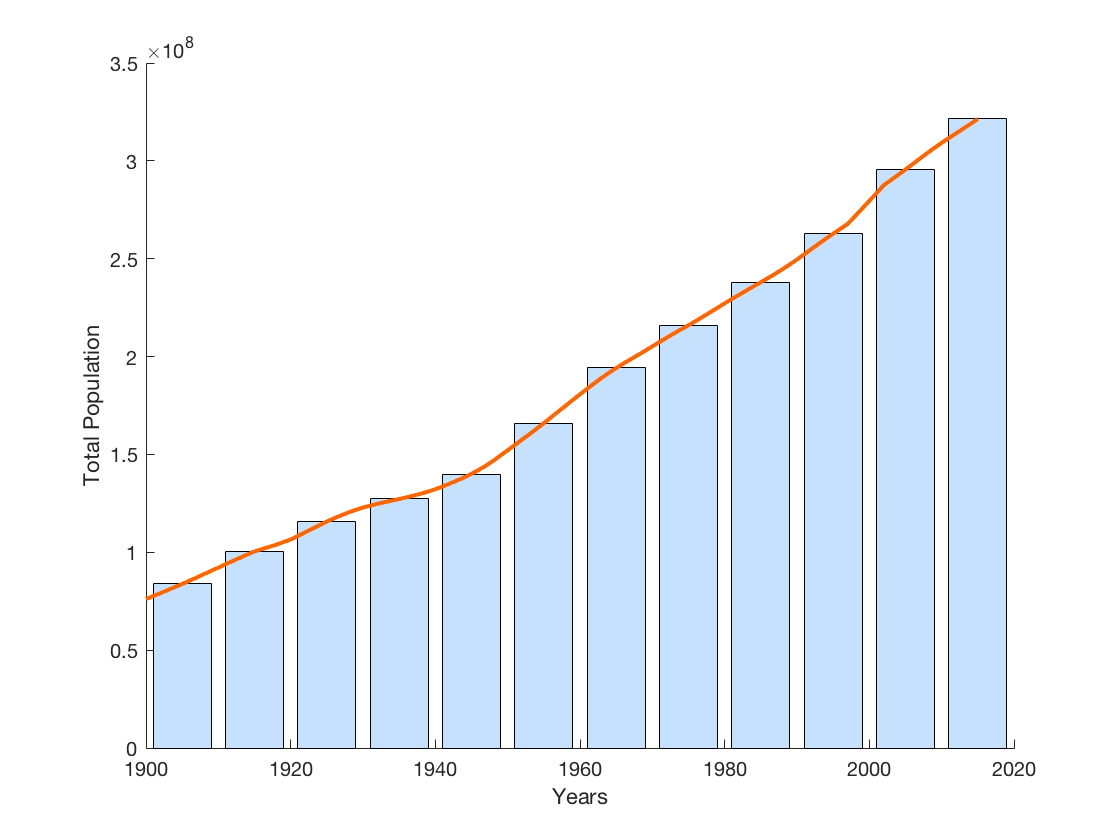
\includegraphics[width=0.7\textwidth,keepaspectratio]{images/us-population}
\caption{US Population zwischen 1953 und 2015}
\label{fig:us-population}
\end{figure}

Die US Populationsentwicklung ist in Abbild \ref{fig:us-population} zu sehen. Die durchschnittliche Rate ist der orangenen Linie zu entnehmen. Es ist ein stettiges Wachstum auf ein level zugehend von 320 Millionen im Jahr 2015.

\subsection{SEEIR MDR-TB Modell}

Im ersten Experiment wurde versucht das Modell von \cite{Trauer2014} in Matlab zu implementieren. Das Reproduzieren, ist aufgrund der menge, an Differentialgleichungen und Parametern nicht trivial. Das System inkorperiert MDR-TB und ist in zwei größere Gruppen eingeteilt. Das Modell von \cite{Trauer2014} ist in Abbildung \ref{fig:mdr-tb-model} zu sehen.

\begin{minipage}{0.4\linewidth}
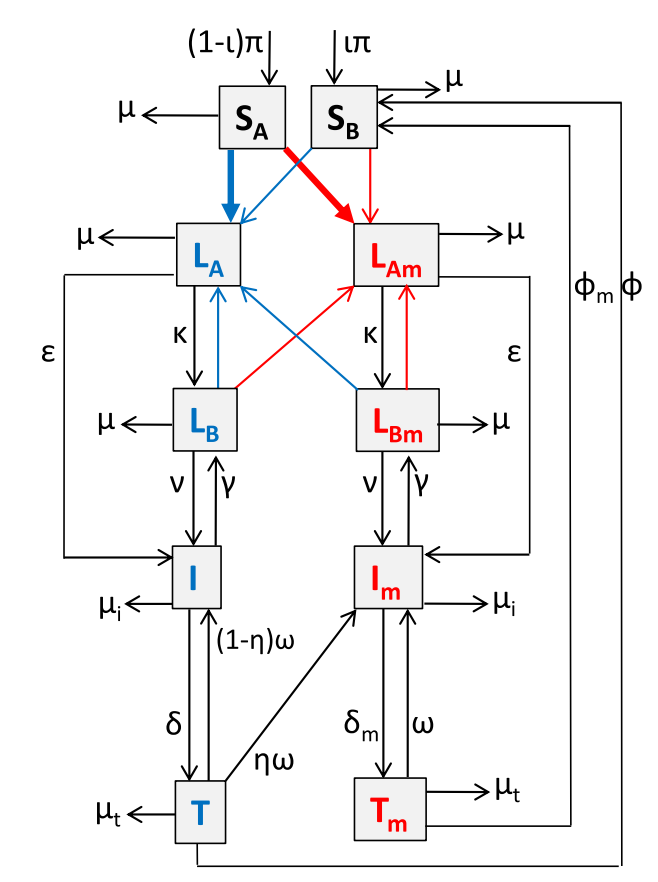
\includegraphics[width=\linewidth]{images/mdr_tb_model}
\label{fig:mdr-tb-model}
\end{minipage}\hfill
\begin{minipage}{0.55\linewidth}
Das Modell ist in zwei Systeme aufgeteilt mit kleinen Übergängen zwischen diesen Systemen. Die Differentialgleichungssysteme beschreiben ein klassisches SEIR Modell mit einer latenten Phase mehr. $L_{A}$ ist die erste latente Phase, wo die Wahrscheinlichkeit auf Erkrankung geringer ist als bei der aktiveren Phase $L_{B}$. Die Autoren haben herausgefunden das eine Modellierung so besser abzubilden ist. Das Differentialgleichungssystem was aus $S_{A}$ folgt, stellt das Transfer Diagramm der herkömmlichen TB dar. $S_{B}$ hingegen stellt die MDR-TB dar mit höheren Ressistenzen. Es ist festzustellen das $\mu$ die Sterberate ist. $\phi$ hingegen beschreibt den Übergang von einer Genesung, direkt in die anfällige Gruppe der MDR-TB. Ferner gibt es einen Rückfallfaktor $\eta \omega$ nach Genesung von $T$ zu $I_{m}$ direkt in die MDR-TB.
\end{minipage}\\\\

Das obige Transfer Diagramm wird als Differentialgleichungssystem realisiert und sieht wie folgt aus

\begin{equation}
\begin{split}
\frac{dL_{A}}{dt} &= \lambda S_{A} + \lambda_{d}(S_{B} + L_{B} + L_{Nm}) - (\epsilon + \kappa + \mu)L_{A} \\
\frac{dL_{Am}}{dt} &= \lambda_{m} S_{A} + \lambda_{dm}(S_{B} + L_{B} + L_{Nm}) - (\epsilon + \kappa + \mu)L_{Am} \\
\frac{dL_{B}}{dt} &= \kappa L_{A} + \lambda I - (\lambda_{d} + \lambda_{dm} + \nu + \mu) L_{B} \\
\frac{dL_{Bm}}{dt} &= \kappa L_{Am} + \lambda I_{m} - (\lambda_{d} + \lambda _{dm} + \nu + \mu) L_{Bm} \\
\frac{dI}{dt} &= \epsilon L_{A} + \nu L_{B} + (1 - \eta)\omega T - (\gamma + \delta + \mu_{i})I \\
\frac{dI_{m}}{dt} &= \epsilon L_{Am} + \nu L_{Bm} + \eta \omega T + \omega T_{m} - (\gamma + \delta_{m} + \mu_{i})I_{m} \\
\frac{dT}{dt} &= \delta I - (\varphi + \omega + \mu_{t}) T \\
\frac{dT_{m}}{dt} &= \delta _{m} I_{m} - (\varphi _{m} + \omega + \mu_{t}) T_{m}
\end{split}
\label{eq:dgls-mdr-tb}
\end{equation}

Wie zuvor auch ist die Populationszahl $N = S_{A} + S_{B} + L_{A} + L_{B} + L_{Am} + L_{Bm} + I + I_{m} + T + T_{m}$ errechnet durch alle Variablen zum Zeitpunkt $t$. Die spezifischen $\lambda$ Parameter kontrollieren die Übergänge zwischen den $S$ und $L$ Klassen, also quasi die latente Infektion.

\begin{gather*}
\lambda = \beta \rho (I + oT)) \/ N \\
\lambda _{d} = \beta_{m} \rho (I_{m} + oT_{m})) / N \\
\lambda _{dm} = \chi\beta_{m} \rho (I_{m} + oT_{m})) / N \\
\end{gather*}

Die eingestellten Parameter für dieses Modell sind im Folgenden aufgelistet und nahe an \cite{Trauer2014} angelehnt.

\begin{table}[ht]
\centering
\small
\resizebox{\textwidth}{!}{
\begin{tabular}{|c|c|c|}
\hline
Variable & Wert & Beschreibung \\
\hline
\multicolumn{2}{|c}{Infektionsparameter} & \multicolumn{1}{c|}{} \\
\hline
$\epsilon$ & 0.129 & Early progression - Diel et al. (2011) \\
$\kappa$ & 0.821 & Transition to late latency \\
$\nu$ & 0.075 & Reactivation - Blower et al. (1995) \\
$\gamma$ & 0.63 & Spontaneous Recovery - Tiemersma et al. (2011) \\
$\mu _{i}$ & 0.37 & TB death rate \\
$\mu _{t}$ & $0.5 \cdot \mu _{i}$ & Treated TB death rate - Harries et al. (2001) \\
$\eta$ & 0.035 & Amplification - Cox et al. (2007) \\
$o$ & 0.21 & Treatment modification of infectiousness - Fitzwater et al. (2010) \\
$\chi$ & 0.49 & Partial immunity - Colditz et al. (1994) \\
$\phi$ & 2 & Drug susceptible treatment rate per year - WHO (2010) \\
$\phi _{m} $ & 0.5 & MDR-TB treatment rate per year \\
\hline
\multicolumn{2}{|c}{Populationsparameter} & \multicolumn{1}{c|}{} \\
\hline
$\pi $ & 0.025 & Birth rate during sensivity Analysis - UNDESA \\
$\mu $ & 0.016 & TB-free mortality - WHO (2013b) \\
$\rho $ & 0.35 & Infectious propertion - WHO (2013c) \\
\hline
\multicolumn{2}{|c}{Kontrollparameter} & \multicolumn{1}{c|}{} \\
\hline
$\iota $ & 0.65 & BCG vaccination rate - World Bank (2013) \\
$\delta $ & 0.65 & Detection rate - WHO (2013c) \\
$\delta _{m}$ & 0 & MDR-TB detection \\
$\omega $ & 0.25 & Default rate - WHO (2013c) \\
$\beta $ & 0.25 & Effective contact rate \\
$mdr$ & 0.06 & proportion of cases MDR-TB 4-6\% \\
\hline
\end{tabular}}
\label{table:mdr-tb-parameters}
\end{table}

Die Resultate des Modells sind unscheinbar. Sobald es zwei Populationen gibt mit TB und MDR-TB, überwiegt die Infektionsrate von MDR-TB.
Das liegt daran, dass es mehr Eingänge zu dem System des MDR-TB gibt und aus der MDR-TB nur geringe Abläufe sind. Es ist zu beobachten, dass ein geringer Anteil der Population in einen Heilungsprozess kommt. Durch fehlende Geburtenrate sind zum Ende des berechneten Zeitraums fast alle Individuen durch die Mortalitätsrate $\mu$ gestorben. Hier fehlt ein System, das sich theoretisch auf einem Equlibrium einpendelt bzw. wo die Krankheitsausbreitungen deutlich geringer sind.

\begin{minipage}{0.6\linewidth}
  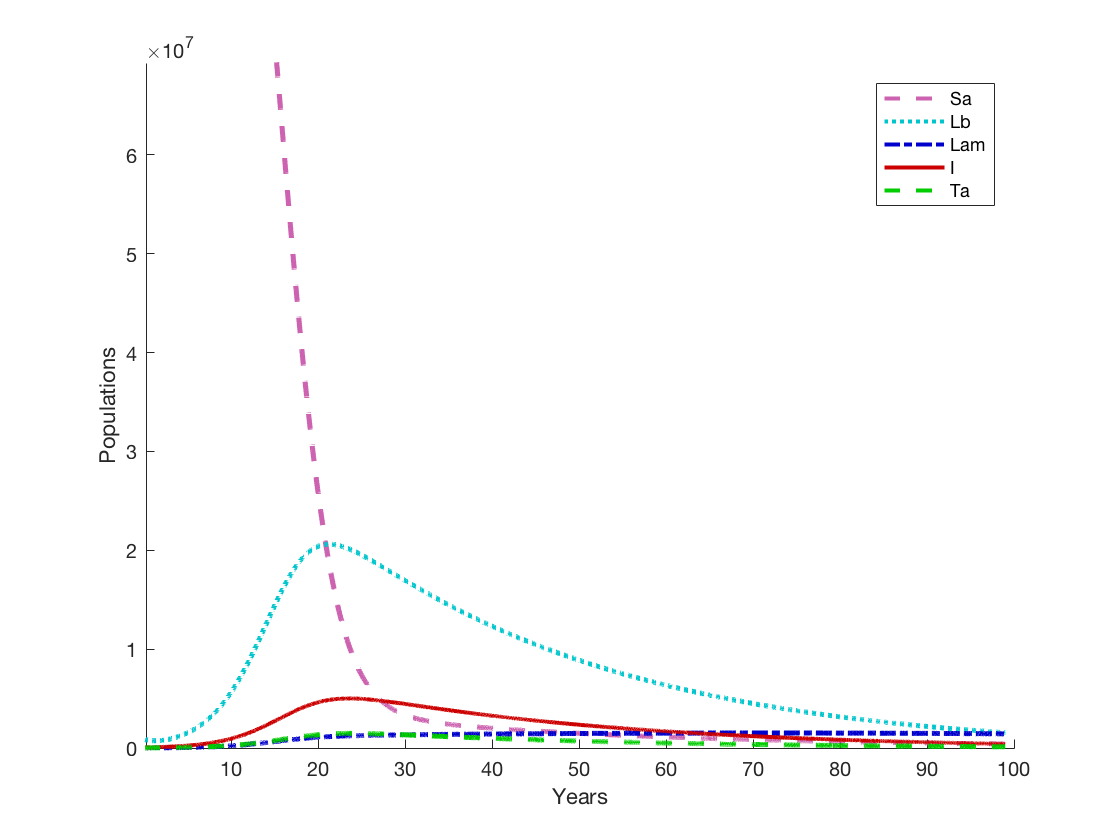
\includegraphics[width=\linewidth]{images/mdr_tb_1}
  \label{fig:mdr-tb-1}
\end{minipage}\hfill
\begin{minipage}{0.4\linewidth}
  Alle Geheilten $T$ sind direkt in die Klasse $S_{B}$ gekommen. Es ist zu beobachten das die empfänglichen enorm schnell abnehmen und zeitgleich latent infizierte übermäßig stark zunehmen. Die Infizierten wiederrum nehmen erst stark zu und dann ab. Die Heilung von Tuberkulose läuft gegen 0.
\end{minipage}\\\\

\begin{minipage}{0.4\linewidth}
  In Abbild \ref{fig:mdr-tb-2} hingegen ist zu beobachten das die empfänglichen leicht zunehmen und latent infizierte extrem zunehmen. Diese kommen aus der Gruppe ohne MDR-TB. Vor allem die Gruppe der langfristig infizierten nimmt zu. Der Trend aller Kurven nach unten ist durch die Sterberate $\mu$ zu begründen. Die infizierten wiederrum sind deutlich geringer, nehmen aber über Zeit zu.
\end{minipage}\hfill
\begin{minipage}{0.6\linewidth}
  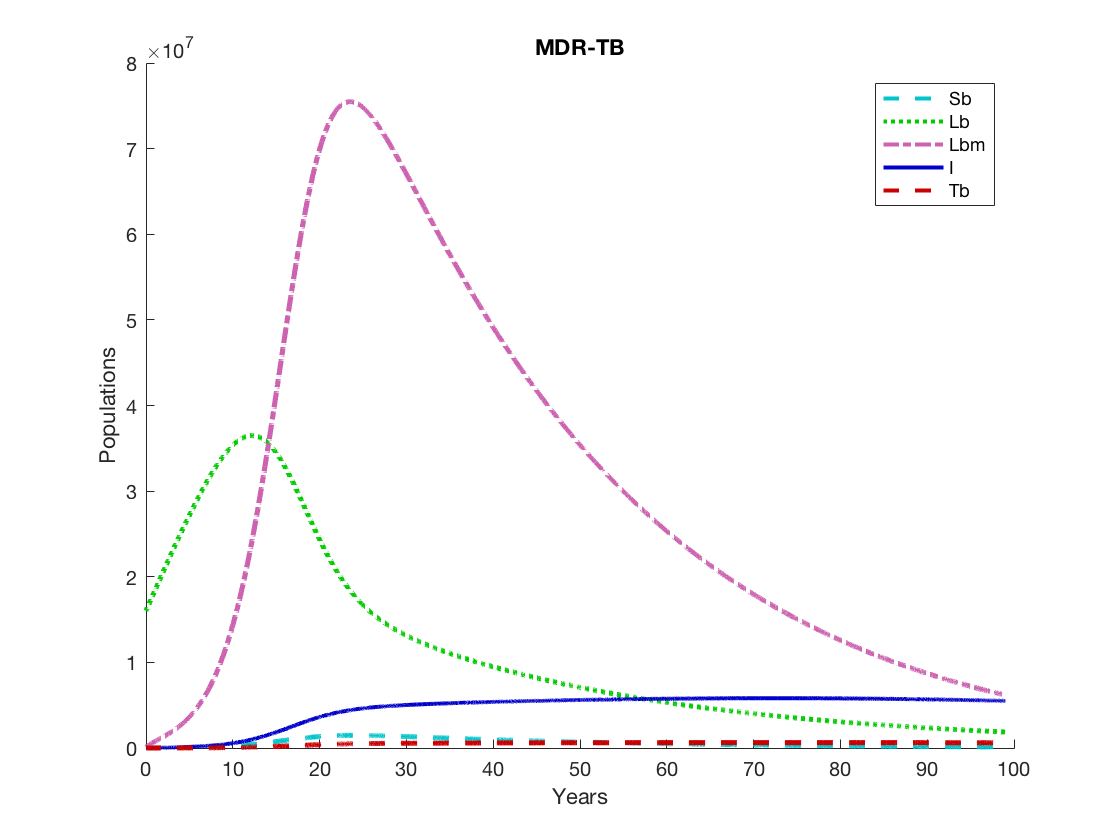
\includegraphics[width=\linewidth]{images/mdr_tb_2}
  \label{fig:mdr-tb-2}
\end{minipage}

Durch diese Art der Modellierung kann durch Variationen der Parameter geschaut werden was effiziente Strategien wären um TB in dieser Simulation einzudämmen. Dies ist in diesem Fall leider nicht gelungen. Die Approximation von optimalen Parametern ist nicht analytisch lösbar und erfordert einiges an mathematischen Anstrengungen.

\subsection{Clustered SELEIR Modell}

Das Clustered SELEIR Modell aus \cite{ModellingTBEpidemics2009} arbeitet mit zwei Populationen $N_{1}$ und $N_{2}$. Das Transfer Diagramm \ref{fig:clustered-seleir} zeigt einige Ähnlichkeiten zu den bisherigen Compartment Modellen, allerdings deutlich komplexer. Um alles schwieriger zu machen sind $U$ die Empfänger ($S$), $A$ sind die infizierten ($I$) und $L$ ist eine neue Klasse von latent infizierten Individuen. Wie zuvor gilt der Kreislauf $U \rightarrow E \rightarrow A \rightarrow R$.

\begin{figure}[ht]
\centering
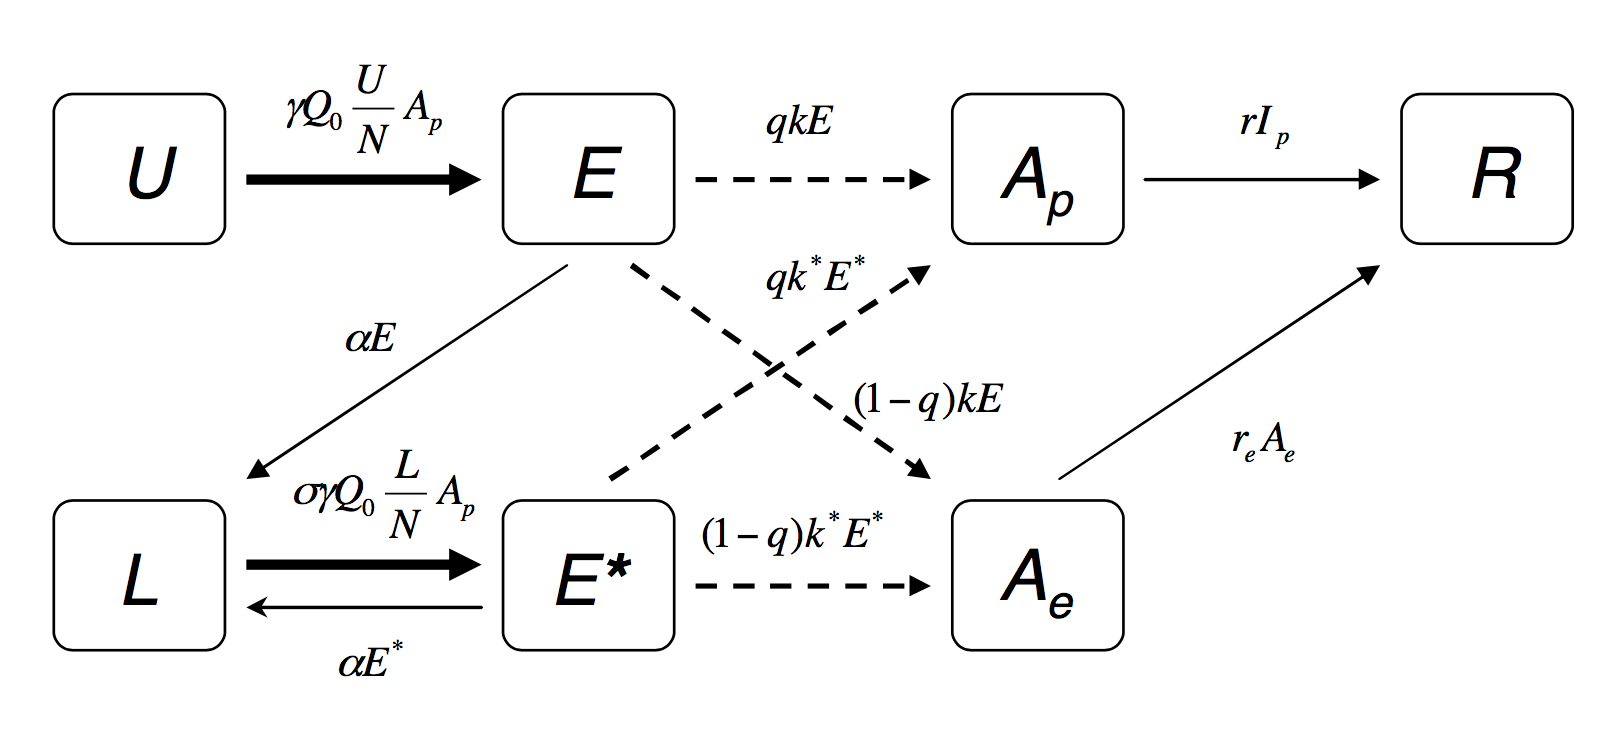
\includegraphics[width=0.9\textwidth,keepaspectratio]{images/clustered_seleir_model}
\caption{Clustered Tuberkulose in \cite{ModellingTBEpidemics2009}}
\label{fig:clustered-seleir}
\end{figure}

Hinzu kommt, dass die latente Phase fein granulärer dargestellt ist. Anstelle von dem direkten Übergang von latent infizierten $E$ zu infizierten gibt es drei Klassen. $E$ kann standardmäßig zur Klasse der Infizierten wandern. Hier gibt es zwei Klassen, der Befall der Lunge ''pulmonale TB'' $A$ oder der Befall anderer Organe ''extrapulmonale TB'' $A^{\*}$. $E$ kann außerdem in die Klasse $L$, lange latente infizierte die eine wesentlich geringere Chance auf den Ausbruch haben. Diejenigen die $L$ mit einer Wahrscheinlichkeit $o\gamma Q_{0}\frac{L}{N}A_{p}$ verlassen sind in einer hochgradig exposierten Variante von $E$, die höhere Wahrscheinlichkeit auf aktiven Ausbruch hat. Wie zuvor werden die Cluster als zwei Populationen in zwei Differentialgleichungssystemen dargestellt. Das Transferdiagramm wird dupliziert und eine explizite Abhängigkeit aufgebaut zwischen diesen erzeugt. Eine generelle Population $N_{1}$ bei der es zufällig mit einem sehr geringen Wert Neuinfektionen für TB gibt. Eine Population mit clustern von erkrankten $N_{2}$ die bei jeder Neuinfektion in $N_{1}$ dahin bewegt wird. Es gibt dann eine Kontaktwahrscheinlichkeit zwischen $N_{1}$ und $N_{2}$. Das volle Differentialgleichungssystem kann in \cite{ModellingTBEpidemics2009} nachvollzogen werden und würde den Rahmen hier sprengen. \\

\begin{figure}[ht]
\centering
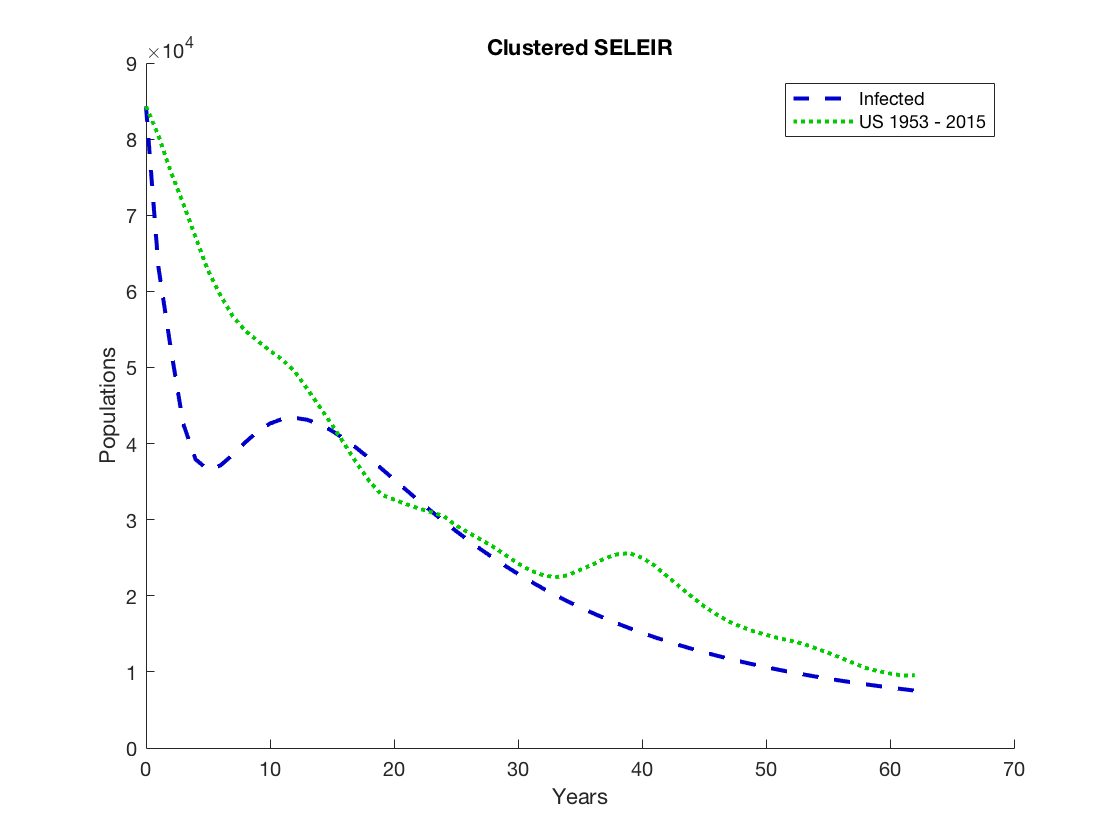
\includegraphics[width=0.8\textwidth,keepaspectratio]{images/clustered_seleir_against_us_data}
\caption{Clustered SELEIR Modell}
\label{fig:clustered-seleir-compare}
\end{figure}

In dem Experiment mit dem Clustered SELEIR Modell ist herauszufinden, wie gut die generellen Populationsparameter für Tuberkulose die Kurve von realen Daten approximieren kann. Das System wurde mit den Bevölkerungsparametern von Tuberkulose aus \cite{Trauer2014} befüllt. Diese Parameter wurden kombiniert mit den Daten der amerikanischen Bevölkerung. In Abbildung \ref{fig:clustered-seleir-compare} sehen wir die Vorhersage des Models über den Zeithorizont in Blau im Vergleich zu der realen Entwicklung in Grün. \\

Es wird relativ klar, das der generelle Trend getroffen wird, die Vorhersagelinie aber nicht der realen folgt. Varianzen in den realen Daten führen nicht zu Varianzen in den synthetisch erzeugten Daten des Modells. Probleme, die hier vor allem auftretten sind die Menge der Parameter. Diese Unschärfe sorgt dafür das es nur durch komplexe analytische Verfahren möglich ist zu bestimmen, inwiefern Parameter angepasst werden müssen. Manche reale Parameter sind zudem nicht bekannt und Parameter sind auch nur als Durchschnitt in diesem Zeitraum statisch.

\section{Agentenbasierte Modellierung zur Ausbreitung von Tuberkulose}

Mit der agentenbasierte Modellierung (ABM) werden Individuen oder Kollektive simuliert und deren Aktionen in einer bestimmten Sichtweise analysiert. Das Ziel ist es neue Erkenntnisse aus den Interaktionsmustern zu entwickeln. Im Vergleich zu den Compartment Modellen ist es bei ABM möglich auch die Lokalität eines Agenten einfließen zu lassen. Ferner lassen sich Agenten auf Schichten platzieren, wobei jede Schicht für unterschiedliche Modellierungsaspekte steht. Es kann z. B. eine Schicht für die physikalischen Interaktionsmuster und Wege existieren und eine andere um die soziale Zusammensetzung zu modellieren. Jede Abstraktionsebene kann getrennt von den anderen Schichten hinzugefügt werden, für die entsprechende Rechenleistung. \\

Im Folgenden wird ein Modell vorgestellt, dass die Ausbreitung von Tuberkulose als ABM realisiert. Hierbei laufen Agenten auf einem Grid per Random Walk. Nur bei direktem Kontakt auf demselben oder umliegenden Grid kann eine Infektion erfolgen. Verschiedenste Bevölkerungsparameter und Übergangswahrscheinlichkeiten wie in Compartment Modellen kommen zum Einsatz. Die Simulation wurde in Python Mesa, einem ABM Framework, geschrieben.

\subsection{Modellierung von Tuberkulose in Mesa}

Mesa ist ein ABM Framework in Python \cite{Mesa}. Es existieren unterschiedliche Funktionalitäten um Agenten auf einem oder mehreren Feldern zu platzieren und mit diesen über einen Zeitraum zu planen. Im Folgenden ein paar Erläuterungen zu dem Mesa Framework und der Modellierung von Tuberkulose. \\

Die \textit{AgentDistribution} hält alle Populationsparameter. Jeder neue Agent wird aus dieser Klasse mit Stichprobenparametern befüllt. Unter anderem kommt hier das Konzept von den Compartment Modellen - $SLIR$ - zum Einsatz um Agenten in einzelne Klassen einteilen zu können. Bei den Ansätzen wurde sich vor allem an dem Modell von \cite{Perez2009} orientiert.

\begin{lstlisting}[style=python]
class AgentDistribution():

  def __init__(self, S=100., L=10., I=1., R=0.):
    pass
\end{lstlisting}

Agenten müssen auf einem Grid platziert werden können. Zu aller erst wird eine neue Stichprobe generiert und ein neuer Agent mit diesen Daten erzeugt. Jeder Agent wird dem Mesa Scheduler hinzugefügt und auf dem Grid platziert. In jedem Update oder Tick wird die Simulation um eine Zeiteinheit $t$ weitergeführt. Der scheduler geht Round Robin alle Agenten durch und kann optimal Populationsdaten einsammeln. Ein Agent bewegt sich aufgrund seiner zu implementierenden \textit{step} Schnittstelle. Dieser \textit{step} wird an alle Agenten propagiert, die dann ihre individuellen Handlungen durchführen.

\begin{lstlisting}[style=python]
from Mesa import Model
from grid import Grid

class DiseaseModel(Model, Grid):

  def __init__(self, agent_dist, width, height):
    Grid.__init__(self, width, height)

    self.number_of_agents = agent_dist.N
    self.time_unit = agent_dist.time_unit
    self.agent_dist = agent_dist
    self.schedule = RandomActivation(self)
    for i in range(self.number_of_agents):
      self.create_agent(unique_id=i)

  def create_agent(self, unique_id=None):
    attributes = self.agent_dist.generate_sample()
    agent = Human(unique_id, self, attributes)
    self.schedule.add(agent)
    self.place_agent(agent)

  def step(self):
    self.schedule.step()
\end{lstlisting}

Der Mesa Agent besitzt alle nötigen Eigenschaften, um mit anderen Agenten zu kommunizieren und wichtige Lokalitätskriterien abzufragen. Ein spezieller \textit{AAgent} besitzt die Schnittstelle, um beliebige Interaktionen mit dem Mesa Grid und Scheduler zu machen wie z. B. der Random Walk. Der \textit{TBAgent} besitzt dann alle Eigenschaften, um speziellere Aktionen bezüglich der Tuberkulose aufzunehmen. Ein Mensch hat prinzipiell nichts mit TB zutun, weshalb dieser dann eine Unterkategorie des \textit{TBAgent} darstellt. Der Mensch kann sich Reproduzieren, Sterben, Altern, TB entwickeln/anstecken, impfen, behandeln lassen und sich bewegen.

\begin{lstlisting}[style=python]
import tuberculosis as tb

from mesa import Agent

class AAgent(Agent):

  def __init__(self, unique_id, model):
    Agent.__init__(self, unique_id, model)

class TBAgent(AAgent):

  def __init__(self, unique_id, model):
    AAgent.__init__(self, unique_id, model)

  def subsceptible(self):
    return tb.subsceptible(self.state)

  def infected(self):
    return tb.infected(self.state)

class Human(TBAgent):

  def __init__(self, unique_id, model, attrs):
    TBAgent.__init__(self, unique_id, model)

    self.age = attrs['age']
    self.birth = attrs['birth']
    # ...

  def step(self):
    self.move()
    self.aging()
    self.reproduce()
    state = tb.next_state(self)
    self.update_state(state)
    self.chance_of_death()
\end{lstlisting}

Das Tuberkulose Modell beinhaltet alle Parameter zur Tuberkulose und die Berechnung der Infektions- und Übergangswahrscheinlichkeiten. Jeder \textit{Human} Agent muss daher bestimmte Attribute wie Alter, HIV-positiv/negativ, Impfung, weitere Immunerkrankungen, TB Behandlung/Therapie und die Lebenserwartung initialisiert bekommen. Es müssen weitere Schnittstellen erfüllt sein um die Lokalität des Agenten und der herumliegenden Agenten abzufragen.

\begin{lstlisting}[style=python]
def next_state(h):
  state = h.state

  if h.vaccinated:
    return R

  aging_chance = aging(h.age, h.le)

  if state == S:
    if infect(h.inf_cm(), h.inf_nb()):
      state = SState(h.hiv, h.immune_diseases, aging_chance)

  elif state == L:
    state = LState(h.treatment, h.hiv, h.immune_diseases, aging_chance)

  elif state == I:
    state = IState(h.treatment, h.hiv, h.immune_diseases, aging_chance)

  elif state == R:
    if infect(h.inf_cm(), h.inf_nb()):
      state = RState(h.treatment, aging_chance)

  else:
    raise Exception("'state={}' must be in {}!".format(state, ", ".join(STATES)))

  return state
\end{lstlisting}

Impfung führt immer zu $R$, nur im $S$ oder $R$ Status kann ein Agent infiziert werden. Diese Wahrscheinlichkeit wird durch $infect$ berechnet, wodurch überhaupt determiniert wird ob es eine Ansteckungsgefahr gibt. Die Ansteckungsgefahr wird durch die umliegenden, aktiv infizierten Agenten berechnet. Nicht jeder direkte Kontakt führt zu einem neuen Infekt. Danach wird berechnet, aufgrund der Agentenparameter, wie wahrscheinlich ein Agent in das latente oder aktive TB Stadium läuft. \\

Zu guter Letzt kann die Simulation über ein Backend Server abgerufen werden. Hierbei bindet Mesa sich an eine konfigurierte IP, standardmäßig 127.0.0.1 auf einem festgelegten Port z. B. 9000. Über z. B. einen Browser kann dann über \textit{http://127.0.0.1:9000} auf die Simulations-GUI zugegriffen werden. In Abbildung \ref{fig:mesa-grid} ist das Simulationsgrid zu erkennen, wobei $S$, rund und Blau, $R$, rund und Grün, $L$, rechteckig und Gelb und $I$, rechteckig und Rot, ist. In Abbildung \ref{fig:n-population} ist die Gesamtpopulation zu sehen. Dabei ist auf der y-Achse die Bevölkerungsanzahl und auf der x-Achse der Zeitpunkt $t$ zu sehen.

\begin{figure}[ht]
  \centering
  \begin{subfigure}{.5\textwidth}
  \centering
  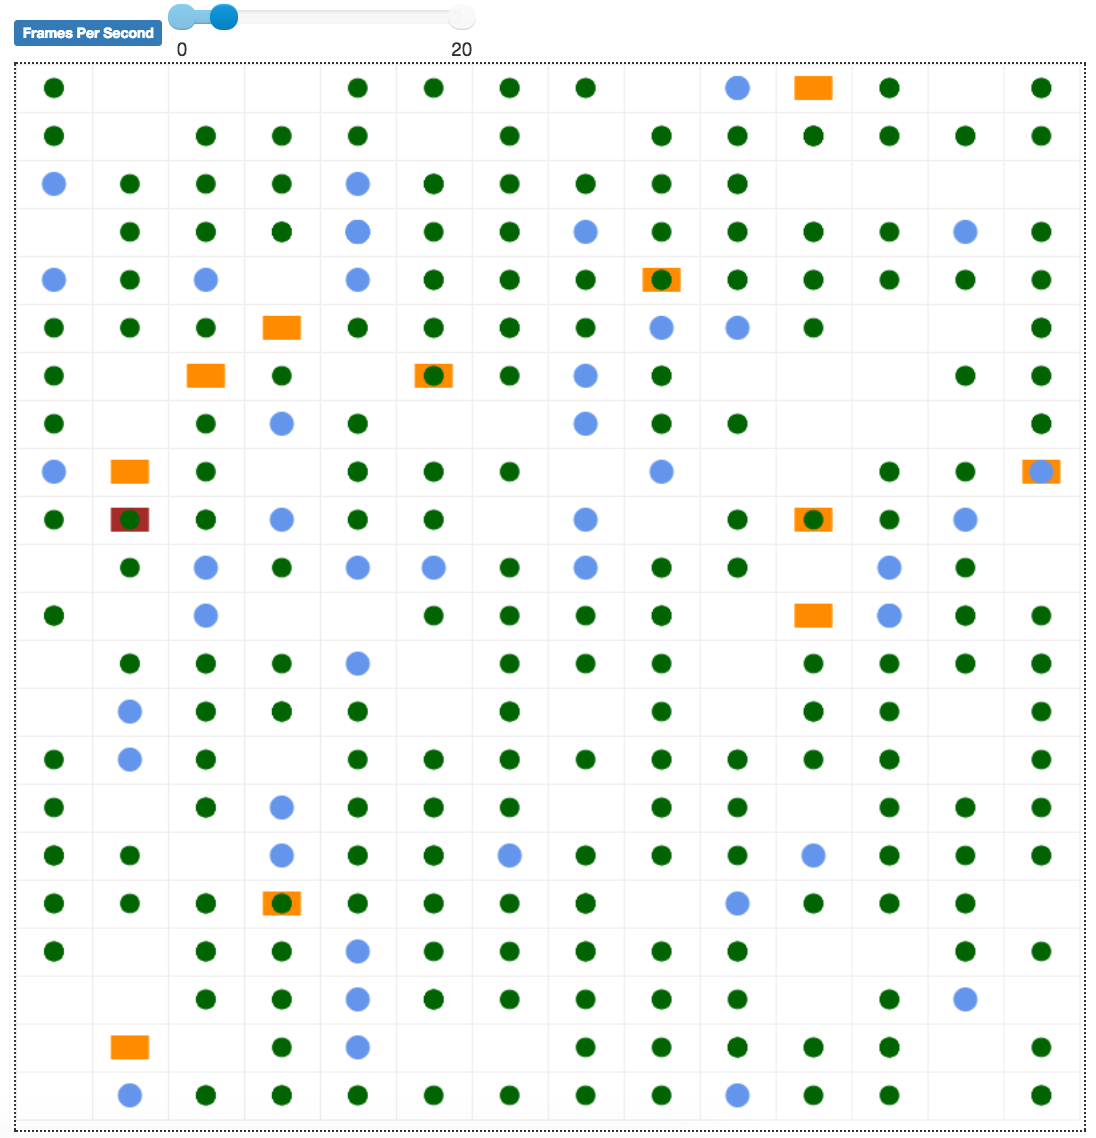
\includegraphics[width=.99\linewidth]{images/mesa-grid}
  \caption{Das Mesa Grid}
  \label{fig:mesa-grid}
\end{subfigure}%
  \begin{subfigure}{.5\textwidth}
  \centering
  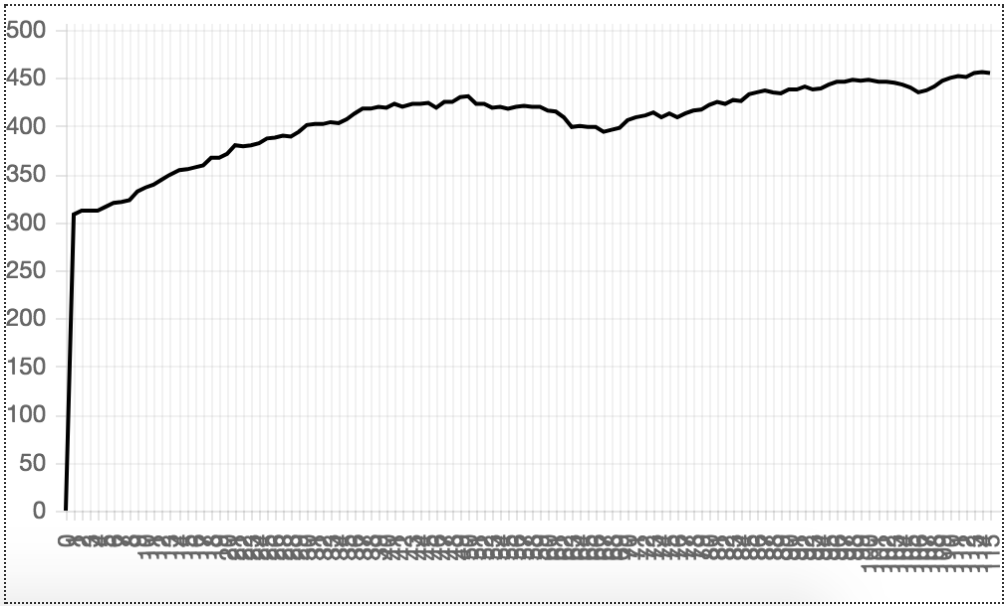
\includegraphics[width=.99\linewidth]{images/n-population}
  \caption{Die Gesamtpopluation $N = S + L + I + R$}
  \label{fig:n-population}
  \end{subfigure}
\end{figure}

Die Populationskomposition, daher $N = S + L + I + R$ kann in Abbildung \ref{fig:l-i-population}, für $L$ und $I$, sowie in Abbildung \ref{fig:s-r-population}, für $S$ und $R$ beobachtet werden. Die Simulation ist in Jahren und wurde auf der x-Achse über ca 100 Jahre geführt.

\begin{figure}[ht]
  \centering
  \begin{subfigure}{.5\textwidth}
  \centering
  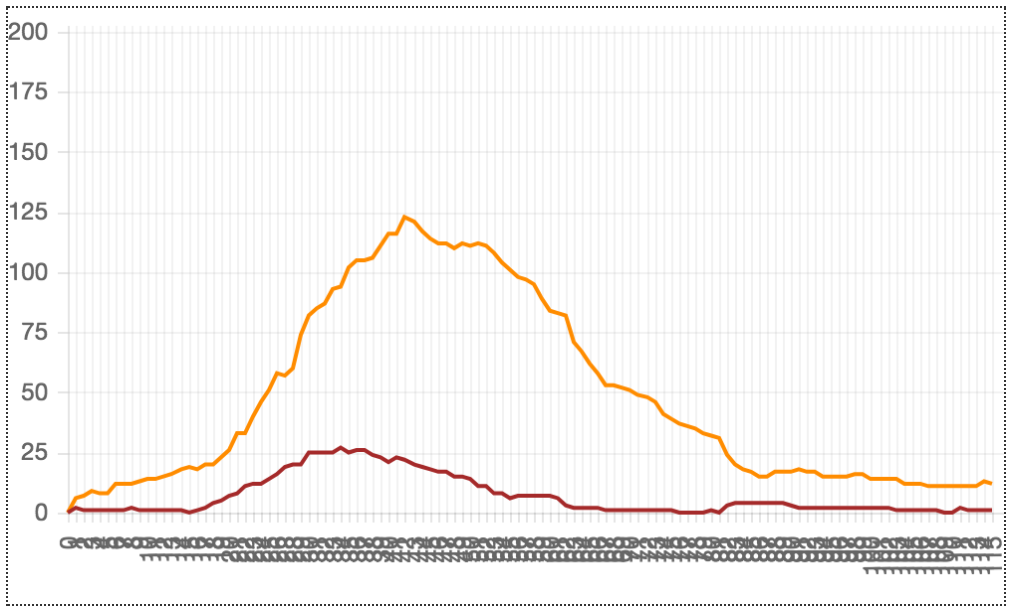
\includegraphics[width=.99\linewidth]{images/l-i-population}
  \caption{Die Popluationen $L$ und $I$}
  \label{fig:l-i-population}
  \end{subfigure}%
\begin{subfigure}{.5\textwidth}
  \centering
  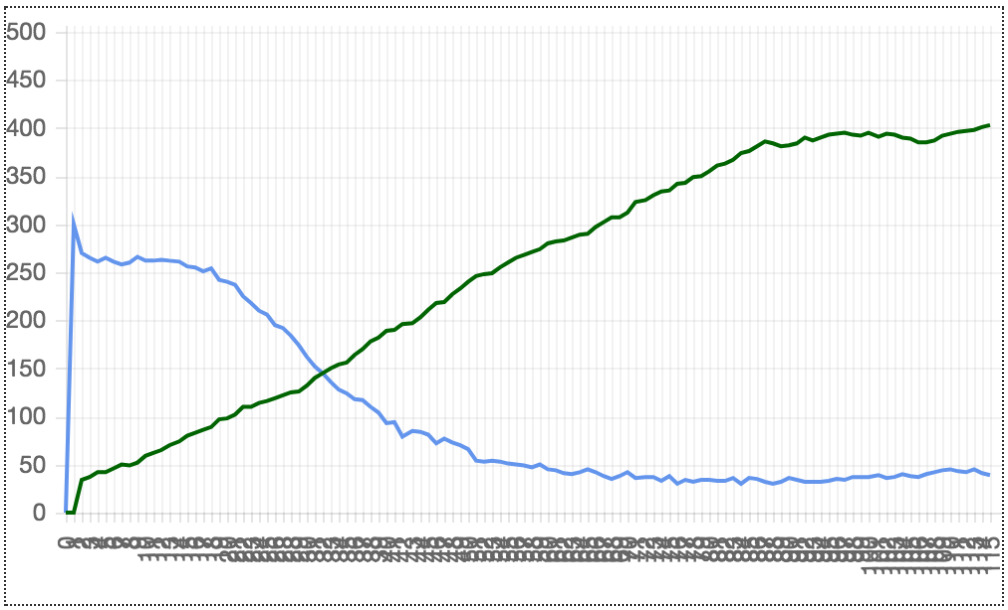
\includegraphics[width=.99\linewidth]{images/s-r-population}
  \caption{Die Popluationen $S$ und $R$}
  \label{fig:s-r-population}
  \end{subfigure}
\end{figure}

\subsection{Eigenschaften des Modells}

Das vorliegende ABM Modell in Mesa, ist nahe angelehnt an Compartment Modelle. Dabei werden ein paar stochastische Eigenschaften von Distributionen ausgenutzt und mit Effekten kombiniert, die durch direkten Kontakt hervorgerufen werden. Des Weiteren werden Parameter vorgestellt und ein paar Experimente beschrieben. Für das Ziehen von Stichprobendaten wurden Funktionen aus Python $numpy$ verwendet. Zum Ziehen von binären Events wurde die Binominal Distribution mit einem wahrscheinlichkeitsparameter genutzt. Die formale Definition der Binominal Distribution ist

\begin{gather*}
P(k; n, p) = P(X = k) = \binom{n}{k}p^{k}(1 - p)^{n - k} \\
\binom{n}{k} = \frac{n!}{k!(n-k)!}
\end{gather*}

Die Binominaldistribution eignet sich für Stichproben die aus einem diskreten Raum kommen. Es wird dann eine Distribution mit $0$ und $1$ aufgestellt, wobei $0$ für keine Ausprägung und $1$ für eine Ausprägung steht. Diese Ausprägungen werden dann über einen Parameter $p$ mit Anteilen belegt. Die resultierende Binominaldistribution zieht dann Stichproben mit einer Wahrscheinlichkeit, dass der Wert $0$ ist mit $p$ und die Restwahrscheinlichkeit, dass der Wert $1$ ist. Interessanter wird es mit der Gamma Distribution. Das Alter einer Bevölkerung lässt sich beispielsweise wie in Abbildung \ref{fig:gamma-age-dist} initialisieren.

\begin{figure}[ht]
  \centering
  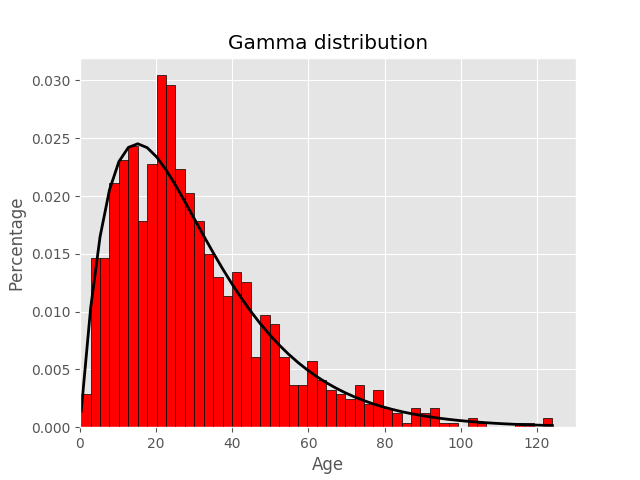
\includegraphics[width=0.8\textwidth,keepaspectratio]{images/gamma-age-dist}
  \caption{Gamma Distribution für Altersverteilungen}
  \label{fig:gamma-age-dist}
\end{figure}

Die vorliegende Bevölkerung ist im Durchschnitt über 10 und unter 40 und die Lebenserwartung einzelner Individuen sehr gering bis ins hohe Alter. Für die Simulation wurden insgesamt folgende Parameter angenommen

\begin{itemize}
\item{Alter - Stichproben aus einer Gamma Distribution}
\item{Geburtenrate - in prozentualen Anteilen per Update (entscheidet darüber, ob ein Agent, Kinder bekommt)}
\item{Impfung - Ob ein Agent geimpft wurde}
\item{Klassen - Die Klasse $S$, $L$, $I$ oder $R$}
\item{Behandlung - Ob ein Agent behandelt wird}
\item{HIV - HIV-positiv/negativ eines Agenten}
\item{Immunkrankheiten - Immunerkrankungen eines Agenten}
\end{itemize}

Außerdem wurden folgende Effekte programatisch berücksichtigt

\begin{itemize}
\item{Neugeborene - Die Geburtenrate entscheidet wieviele Individuen neu erzeugt werden pro Update. Neugeborene sind standardmäßig immer 0 Jahre alt bei der Geburt und bekommen HIV nur dann, wenn die Eltern diese Krankheit auch haben. Ob die Eltern geimpft sind, gibt einen Ausschlag darüber aus, ob Kinder ebenfalls geimpft werden.}
\item{Tod - Individuen sterben am Alter, daher wenn sie die Lebenserwartung aus der Alterdistribution erreichen, steigt die Chance auf Tod. Ferner, gibt es Sterben durch Tuberkulose, sowie eine zufällige Sterberate, die immer eintreten kann.}
\item{Die Umgebung eines Individuums spielt eine Rolle, da mehr Kontakt zu anderen infizierten das Risiko deutlich erhöht. Es gibt auf dem Grid einen Radius der Infektion, der bestimmt, über wieviele Felder die Infizierten andere anstecken können.}
\item{Die Zeit, wenn ein Individuum in der Klasse $E$ ist, wird aufgenommen. Die Wahrscheinlichkeit in Klasse $I$ zu wandern steigt mit fortlaufender Zeit.}
\item{Die Zeit, wenn ein Individuum in der Klasse $I$ ist, wird aufgenommen. Die Wahrscheinlichkeit in Klasse $R$ zu wandern oder zu sterben steigt mit fortlaufender Zeit.}
\end{itemize}

Die Übergangswahrscheinlichkeiten zwischen den Compartments werden anhand einer Markov Kette definiert. Jeder Agent hat nur seine aktuelle Klasse $S$, $L$, $I$ oder $R$. Die Markov Eigenschaft verlangt das

\begin{gather*}
\Pr(X_{n+1}=x\mid X_{1}=x_{1},X_{2}=x_{2},\ldots ,X_{n}=x_{n})=\Pr(X_{n+1}=x\mid X_{n}=x_{n}) \\
\Pr(X_{1}=x_{1},\ldots,X_{n}=x_{n}) > 0
\end{gather*}

Das heißt, der nächste Zustand $x_{n + 1}$, daher z. B. die Übergangswahrscheinlichkeit das $x_{n} = L$ in die Klasse $x_{n + 1} = I$ läuft, ist nur bedingt durch den derzeitigen Zustand $x_{n}$. Das heißt konkret das $x_{n-1}, x_{n-2}, \ldots, x_{1}$ keine Rolle spielen. Nach der Bayesianischen Forderung wollen wir im Prinzip aus dem aktuellen Wissen ''prior'' und neuen Beobachtungen eine neue Erkenntnis ''posterior'' finden. Jeder Agent wird dadurch simuliert wie viele der anderen Agenten sich in den einzelnen Klassen befinden. Durch die individuellen Ausprägungen eines Agenten und durch die Übergangswahrscheinlichkeiten der oben beschriebenen Markov Kette, wird die Wahrscheinlichkeit vom Übergang in ein anderes Compartment berechnet.

\[
M=
  \begin{bmatrix}
    .95 & .05 & .0 & .0 \\
    .0 & .9 & .1 & .0 \\
    .0 & .1 & .7 & .2 \\
    .0 & .45 & .05 & .5 \\
  \end{bmatrix}
  \begin{tabular}{c}
    \text{S - Empfänger} \\
    \text{L - latent infizierte} \\
    \text{I - infizierte} \\
    \text{R - geheilte}
  \end{tabular}
\]

Die Markov Kette für Übergangswahrscheinlichkeiten in Kombination mit den folgenden Parametern stellt das komplette Modell dar.

\begin{table}[ht]
\centering
\small
\resizebox{\textwidth}{!}{
\begin{tabular}{|c|c|c|}
\hline
Variable & Wert & Beschreibung \\
\hline
\multicolumn{2}{|c}{Distributionen und Initialisierung} & \multicolumn{1}{c|}{} \\
\hline
$S$ & 100 & Epfänger \\
$L$ & 10 & Latent infizierte \\
$I$ & 1 & infizierte \\
$R$ & 0 & geheilte \\
Alter & $Gamma(k=2.0,\theta=15, N=N)$ & Alter, Formparameter $k$ und Skalierungsparameter $\theta$ über die Population $N$ \\
Lebenserwartung & $80$ & Normalverteilung um $80$ herum mit Varianz von $10$ \\
geimpft & $0.1$ & geimpfte Teile der Bevölkerung \\
Geburtenrate & $0.013$ & Wahrscheinlichkeit auf Neugeburt pro Tick \\
HIV & $0.1$ & Wahrscheinlichkeit auf HIV bei Initialisierung und Neugeburt \\
Behandlung & $0.3$ & Wahrscheinlichkeit auf HIV Behandlung bei Erkrankung \\
Immunkrankheiten & $0.2$ & Wahrscheinlichkeit auf Immunerkrankung bei Initialisierung oder Neugeburt \\
\hline
\multicolumn{2}{|c}{Lokalitätsparameter} & \multicolumn{1}{c|}{} \\
\hline
Infektionsradius & $5$ & Reichweite der Ansteckungsgefahr sind $5$ Felder \\
Bewegungsweite & $1$ & Schritt pro Agent pro Tick. \\
Moore + Center & $True$ & Diagonale zählen als Nachbarn + mehrere Agenten auf einem Platz \\
Infektionsrisiko Center & $0.3$ & Wahrscheinlichkeit das eine Infektion auftritt wenn Infizierter auf demselben Feld \\
Infektionsrisiko Nachbar & $0.1$ & Wahrscheinlichkeit das eine Infektion auftritt wenn Infizierter auf einem benachbarten Feld \\
\hline
\multicolumn{2}{|c}{Risikoparameter} & \multicolumn{1}{c|}{} \\
\hline
HIV Risiko & $0.4$ & Wahrscheinlichkeit das eine Klasse in die nächste wandert ist ehhört bei HIV \\
Immunkrankheiten Risiko & $0.1$ & Wahrscheinlichkeit das eine Klasse in die nächste wandert ist ehhört bei Immunkrankheiten \\
Behandlung Chance & $0.4$ & Wahrscheinlichkeit das Infizierter geheilt wird ist erhöht \\
Alter Risiko & $\frac{Alter}{Lebenserwartung} \cdot 0.001$ & Wahrscheinlichkeit das eine Klasse in die nächste wandert ist ehört bei höherem Alter \\
\hline
\end{tabular}}
\label{table:agent-parameters}
\end{table}

\subsection{Resultate}

Mit obigen Konfigurationsparametern ist es nun spannend zu beobachten, ob es eine Reihe von Faktoren, gibt die Tuberkulose eindämmen können. Es konnte beobachtet werden, wenn die Impfung bei Neugeborenen der Population deutlich erhöht wird, mit z. B. 60\% aller Neugeborenen, verschwindet TB über einen langen Zeitraum vollständig. Da Infizierte keinerlei Chance auf Heilung besitzen, ist die sinnvollste Strategie bei der nächsten Generation anzufangen. Interessant ist auch das durch das Einführen von MDR-TB, über einen langen Zeitraum alle Menschen gestorben sind, da diese durch die Behandlung von Medikamenten nicht verschwindet. Die Variation von den Lokalitätsparametern hat auch einen großen Einfluss. Es stellte sich heraus das nur größere Radien $> 4$ Felder für eine TB Epidemie sorgen konnten. Kleinere Cluster wurden ebenfalls gebildet. Teile der Bevölkerung waren noch nicht infiziert, während andere Teile schon viele Infizierte vorweisen konnte. Langfristig kann ein stabiles Maß gefunden werden, wenn allein die geimpften Eltern, ihre Kinder ebenfalls impfen wie in den unteren Abbildungen zu sehen ist.

\begin{figure}[ht]
\centering
\begin{subfigure}{.45\textwidth}
\centering
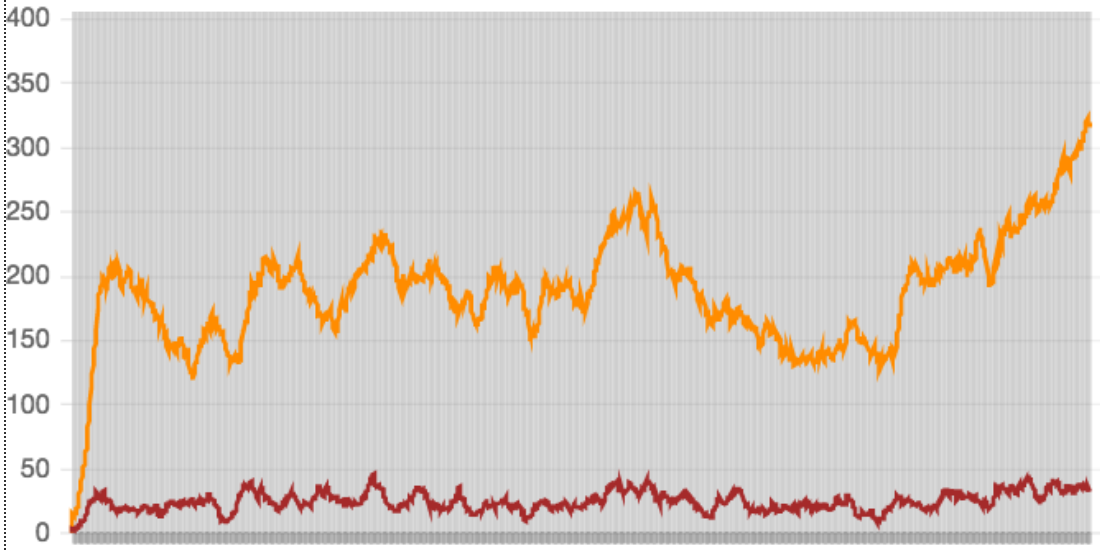
\includegraphics[width=.99\linewidth]{images/abm-l-i-exp-1}
\caption{$L$ (Gelb) und $I$ (Rot)}
\label{fig:abm-l-i-exp-1}
\end{subfigure}%
\begin{subfigure}{.45\textwidth}
\centering
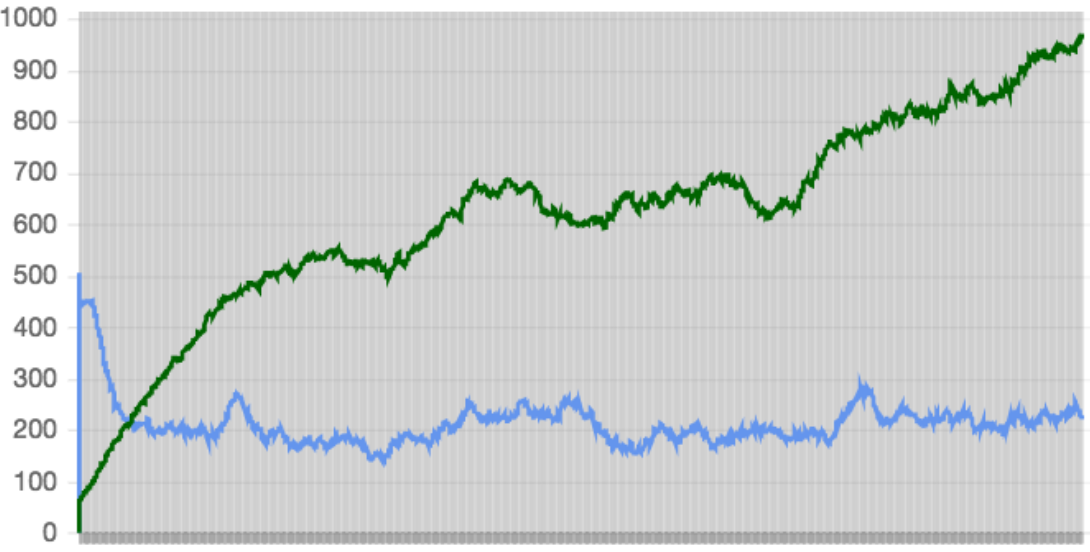
\includegraphics[width=.99\linewidth]{images/abm-s-r-exp-1}
\caption{$S$ (Blau) und $R$ (Grün)}
\label{fig:abm-s-r-exp-1}
\end{subfigure}
\end{figure}
\begin{figure}[ht]
\centering
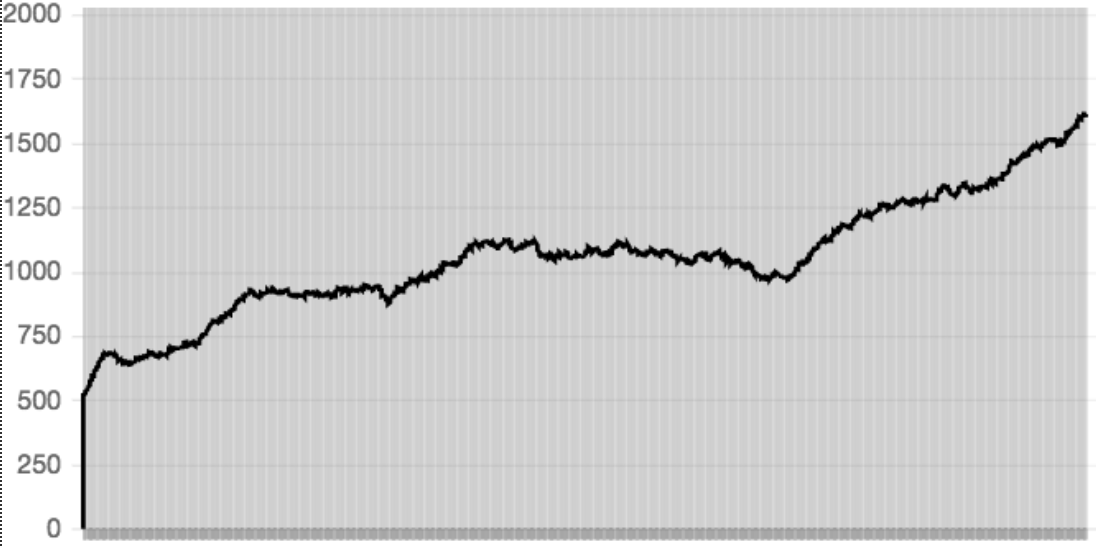
\includegraphics[width=.5\textwidth]{images/abm-n-exp-1}
\caption{Gesamtpopluation $N = S + L + I + R$}
\label{fig:abm-n-exp-1}
\end{figure}

Die Zeitachse ist in kleineren Schritten über 100 Jahre abgebildet. Die Geimpften füllen die $R$ Klasse. Eine höhere Bevölkerung führt zu höheren Anteilen an latenter TB mit periodischen Kurven. Aktiv Infizierte sind relativ gering und gehen periodisch in Schritten rauf und runter.

\newpage

\section{Fazit}

In dieser Arbeit wurde gezeigt, wie agentenbasierte Modellierung und Compartment Modelle genutzt werden können, um die Ausbreitung von Infektionskrankheiten wie Tuberkulose zu simulieren. Idealerweise kommen neue Erkenntnisse ans Licht, wie die Übertragung von Tuberkulose verhindert werden kann. \\

Die beiden Compartment Modelle haben nur geringfügig brauchbare Ergebnisse erzeugt. Auch wenn interessante Effekte zu beobachten waren, können die Ergebnisse nur als plausible Indikatoren für die Ausbreitung von Tuberkulose herangezogen werden. Die agentenbasierte Simulation hat gezeigt, dass unterschiedliche Strategien, zumindest auf synthetisierten Daten, einen Signifikaten Einfluss zur Dämmung von Tuberkulose haben können. Nichtsdestotrotz ist es überaus schwierig relevante Ergebnisse aus diesen Modellen zu bekommen. Dies liegt unter anderem an der enormen Komplexität und der Menge an Variablen die so ein System beeinflussen. \\

Eine der vielversprechendsten Teile der Modellierung mit statistischen Prädiktionsmodellen über eine Menge beschreibender Variablen konnten nicht näher betrachtet werden. Diese Modelle stellen sinnvolle Erweiterungen zu rein theoretischen Modellen dar. Von realen Daten zu lernen beinhaltet den Vorteil, die unterliegenden Trends, deutlich präziser anzunähern. Voraussetzung ist allerdings, dass diese Daten existieren und auch tatsächlich das System von Interesse erklären können.

\newpage

\bibliographystyle{apalike}
\bibliography{md-tuberkulose}

\end{document}
